\section{Theoretical Analysis}
\label{sec:analysis}

\subsection{Central Frequency, Voltage Gain, Input and Output impedances}
Using the equations provided by the professor, we wrote an Octave script in order to compute the following values: central frequency, voltage gain, input impedance and output impedance. \par
Mainly these equations were used:
\begin{equation}
    T(s) = \frac{R_1 C_1 s}{1+ R_1 C_1 s} (1+\frac{R_3}{R_4}) \frac{1}{1+ R_2 C_2 s}
\end{equation}\par
and the same equation described in the simulation section for the central frequency where: \par
\begin{equation}
    Lower_cutoff = \frac{1}{R_1 C_1}
\end{equation}\par
and \par
\begin{equation}
    Upper_cutoff = \frac{1}{R_2 C_2}
\end{equation}\par
The values obtained are in the table below:

\begin{center}
  \begin{tabular}{ | c | c | }
    \hline    
    {\bf Name} & {\bf Value [$Hz$, $dB$ or $\Omega$]} \\ \hline
    \input{../mat/docImp}
    \hline
  \end{tabular}
  \captionof{figure}{Central Frequency, Voltage Gain, Input and Output impedances}
\end{center}

\subsection{Frequency Response}
Taking into account the all circuit, we can obtain the frequency response both in $dB$ and phase:\par

\begin{figure}[H] \centering
\includegraphics[width=0.7\linewidth]{../mat/fresponse1.pdf}
\caption{Frequency Response - $dB$}
\label{fig:fresponse1}
\end{figure}

\begin{figure}[H] \centering
%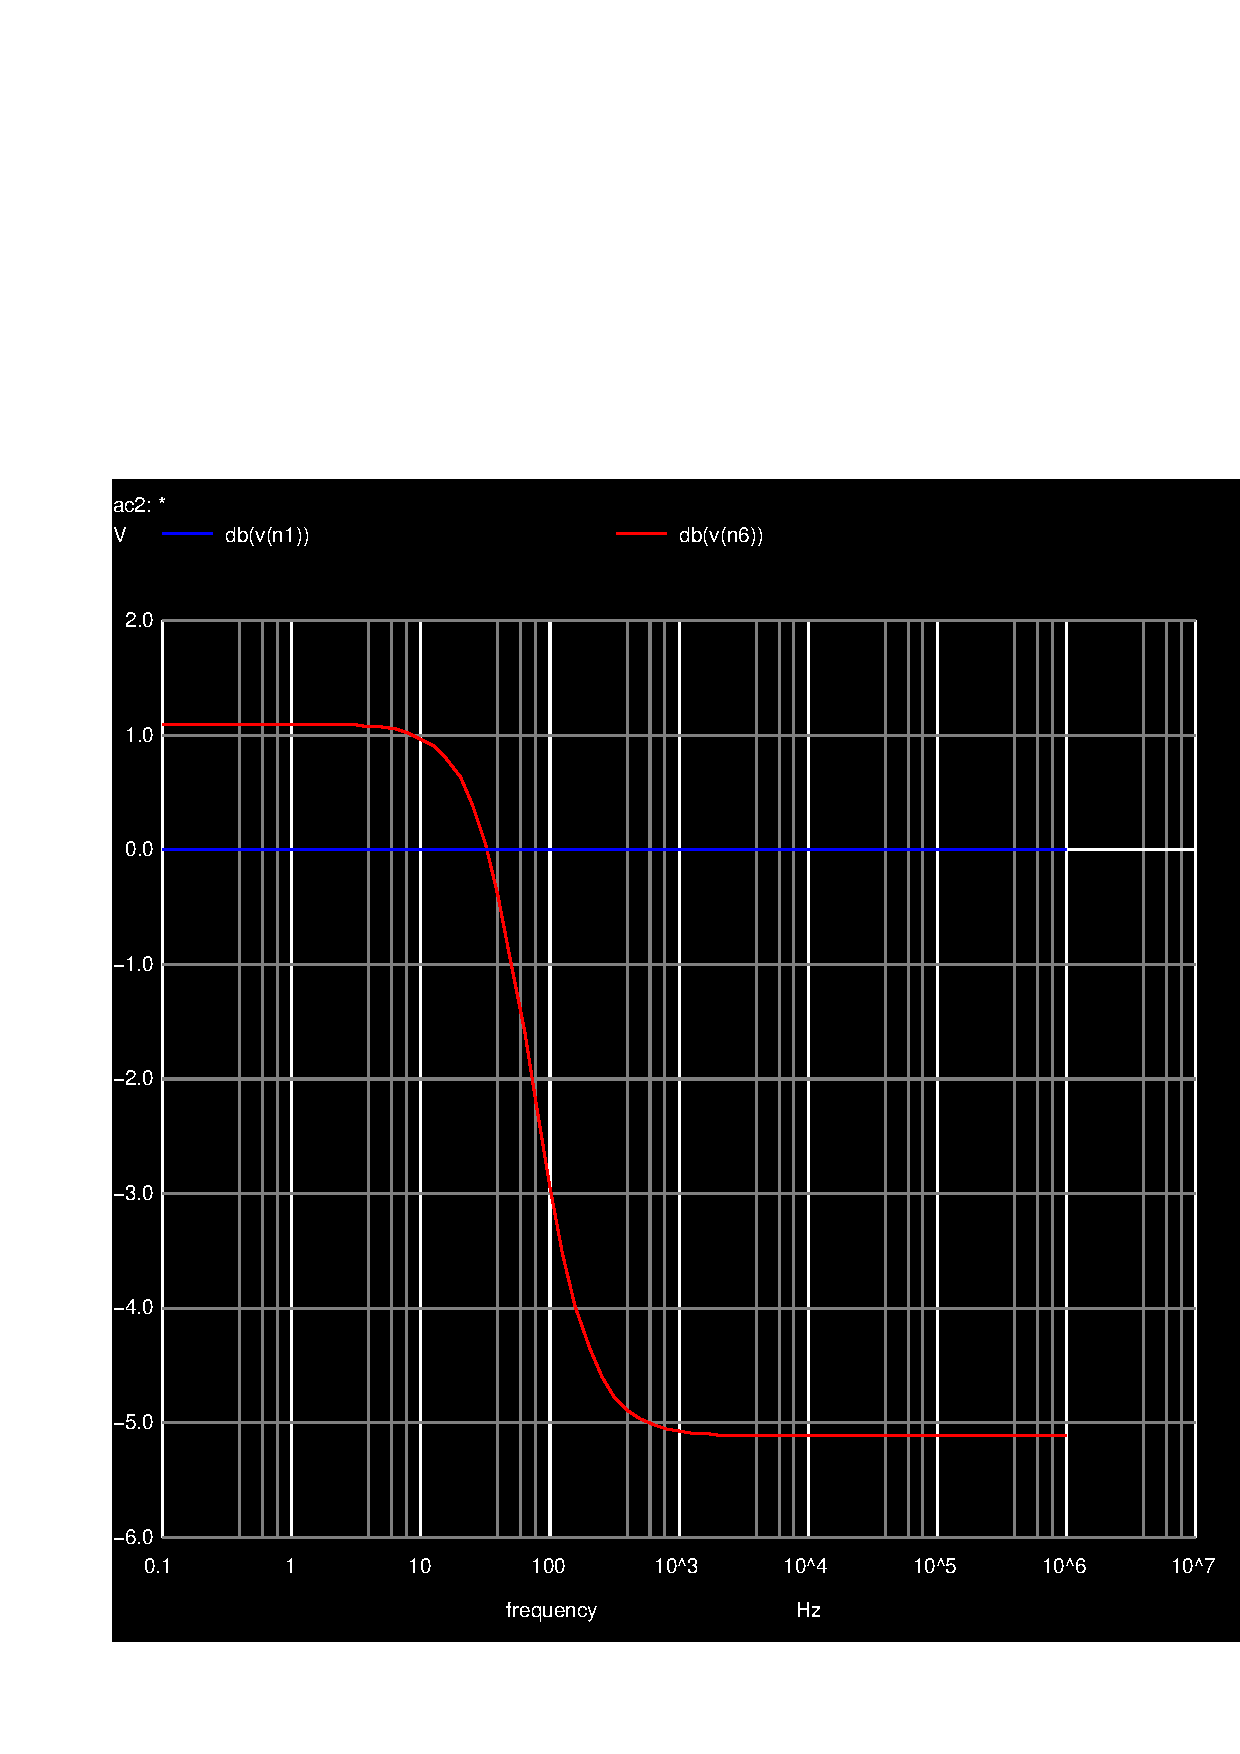
\includegraphics[width=0.7\linewidth]{../mat/fresponse.pdf}
\caption{Frequency Response - Phase}
\label{fig:fresponse2}
\end{figure}
